% This is part of Un soupçon de mathématique sans être agressif pour autant
% Copyright (c) 2015
%   Laurent Claessens
% See the file fdl-1.3.txt for copying conditions.

\begin{exercice}[\ldots\ldots/5]\label{exo2smath-0152}

% Ceci existe dans exo2smath-0175 et exo2smath-0152. L'un pour évaluation et l'autre pour les exercices.
    \begin{multicols}{2}
        Le câble d'un téléphérique mesure \SI{1}{\kilo\meter}  pour monter de \( \unit{600}{\meter}\). Le premier pylône mesure \SI{25}{\meter}.
    \begin{enumerate}
        \item
            Faire un dessin à main levée de la situation.
        \item
    À quelle distance du point de départ faut-il poser le pylône ?
    \end{enumerate}

    \columnbreak
    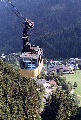
\includegraphics[width=2.5cm]{telepherique.pdf}
    \end{multicols}

\corrref{2smath-0152}
\end{exercice}
